\section{ArchSig: Executable SAGA Diagnosis}\label{sec:7}

ArchSig is a measurement system (a Rust command-line tool) that
computes grounding, derived residuals, boundary membership, comparison
of run pairs, and gate verdicts from two families of inputs:
observation (ArchMap) and law / equations (LawPolicy, law surfaces,
MeasurementProfile). This section first presents a full SAGA diagnosis
of a real microservice architecture as a single computation
(\S\ref{sec:71}--\S\ref{sec:73}), and afterwards fixes the input
contract and the definition of the computation on which the diagnosis
stands (\S\ref{sec:74}). The supply process for observation is fixed in
\S\ref{sec:75}, the kinds of conditions behind the conclusions in
\S\ref{sec:76}, the boundary of the claims in \S\ref{sec:77}, and the
reproduction procedure in \S\ref{sec:78}.

\subsection{A real-code case: the one-cent obstruction}\label{sec:71}

The subject of the case study is the open-source train reservation
system
\href{https://github.com/FudanSELab/train-ticket}{train-ticket}
(commit \code{313886e99bef}, 42 services), widely used as a
microservice benchmark.

On the real call triangle cancel--inside-payment--order of this
system, the three services follow three different conventions for the
refund amount. All three were confirmed in the actual sources and observed as
section values of the ArchMap:
{\sloppy
\begin{itemize}
\item \textbf{cancel}: \code{Double.parseDouble(order.getPrice())}\allowbreak\code{ * 0.8}
rounded by \code{DecimalFormat("0.00")} and rendered as a string
(floating point + rounding);
\item \textbf{inside-payment}: exact arithmetic on
\code{new BigDecimal(order.getPrice())};
\item \textbf{order}: pass-through storage in
\code{private String price}.
\end{itemize}
}

The monetary representations of the three services are all passed as
\code{string} at the implementation level: the types agree. What
differs is the \emph{semantic convention} --- the rounding, scale,
computation, and storage of the amount that the \code{string}
represents. Furthermore, in the source investigation by the operator
(the person executing the measurement process; in this paper, the
author), no site was found that simultaneously reconciles the amounts
of the three services. This investigative finding is reflected in the
diagnosis in the form of declaring no triple overlap in the selected
complex. The absence of a simultaneous reconciliation site is itself
treated as an assertion of the operator, not as a fact exhibited by the
observation artifacts (\S\ref{sec:72}, \S\ref{sec:76}).

This configuration can be read as a 3-cycle instance of the same
\textbf{cycle-without-a-face mechanism} as Example~\ref{ex:circle}.
The complexes are not identical --- Example~\ref{ex:circle} is a
4-cycle, this case a 3-cycle --- but the mechanism erecting the
nonzero class is the same: odd parity on a closed loop (the collision
of three styles) and the absence of a face (triple overlap) filling
the loop. The rounding remainder of the refund computation
$0.8\times\text{price}$ --- a \textbf{drift below one cent} --- is
booked in no chart. We call this case study the \textbf{one-cent
obstruction}.

\paragraph{Semantic trace.}
Table~\ref{tab:semantictrace} fixes the quantities compared by the
three edges and the implementation conventions.

\begin{sidewaystable}[htbp]
\centering
\scriptsize
\begin{tabular}{@{}p{0.10\linewidth}p{0.09\linewidth}p{0.17\linewidth}p{0.13\linewidth}p{0.08\linewidth}p{0.15\linewidth}p{0.16\linewidth}@{}}
\toprule
Edge & Compared quantity & Convention L & Convention R & Normalization
& Expected equation & Witness variable \\
\midrule
cancel--inside-payment & refund amount & the string obtained by
rounding $0.8\times\text{price}$ with \code{DecimalFormat(}\allowbreak\code{"0.00")} &
the exact arithmetic value via \code{BigDecimal} & currency value
(scale-2) & the refund amounts of both charts are determined as the
same currency value & \code{e\_cancel\_insidepay} \\
\addlinespace
inside-payment--order & reference amount of the refund & the exact
value of \code{BigDecimal(}\allowbreak\code{order.}\allowbreak\code{getPrice())} & the pass-through
recorded amount of \code{String price} & currency value (scale-2) &
the reference amount used by payment is determined under the same
convention as the recorded amount & \code{e\_insidepay\_order} \\
\addlinespace
cancel--order & application of the refund ratio & the rounded
$0.8\times\text{price}$ & the recorded amount \code{price} & currency
value (scale-2) & the refund amount is determined uniquely as 0.8
times the recorded amount & \code{e\_cancel\_order} \\
\bottomrule
\end{tabular}
\caption{Semantic trace of the one-cent obstruction: the quantities
compared by the three edges and the implementation conventions.}
\label{tab:semantictrace}
\end{sidewaystable}

What this table fixes is the semantic-grounds side; the residual
values themselves are derived by \code{analyze} from the comparison of
the observed section values of each edge (\S\ref{sec:74}). All three
edges compare restrictions of one and the same semantic quantity ---
the refund amount of this order --- and the degree of freedom of the
mismatch lies along a single direction: under which rounding / scale
convention that quantity is determined as a currency value. The
witness bindings (\S\ref{sec:74}) are the law-side declarations
choosing that direction edge by edge.

\paragraph{Finite witness.}
Separated from any estimate of frequency or total loss (which requires
runtime measurement; \S\ref{sec:77}), we exhibit a witness with one
fixed input price, as a normalization computation applying each
source-confirmed convention to the same refund quantity:
\begin{center}
\footnotesize
\begin{tabular}{@{}ll@{}}
original price: & 12.33\\
cancel convention: & $0.8 \times 12.33 = 9.864$\\
 & $\to$ \code{DecimalFormat("0.00")} $\to$ ``9.86''\\
inside-payment convention: & the same refund quantity by exact
arithmetic\\
 & $\to$ 9.864\\
normalized as currency values: & 9.86 (scale-2) vs.\ 9.864\\
nonzero remainder: & 0.004 (below one cent)\\
\end{tabular}
\end{center}
The multiplication on the cancel side is performed in binary floating
point, but for this input that does not affect the result of the
scale-2 rounding. The remainder violates no chart's local equation ---
cancel is faithful to cancel's rounding convention, inside-payment to
exact arithmetic --- yet it remains as the difference of the values of
the two charts.

This numerical witness is a source-level recomputation by the
operator; none of the price, the $0.8$, the rounding, or the $0.004$
appears in ArchSig's computation.

\subsection{The diagnosis staircase}\label{sec:72}

The measurement inputs are composed as follows (the input contract and
the definition of the computation for each artifact are in
\S\ref{sec:74}).
\begin{itemize}
\item \textbf{cover}: 6 charts --- the diagnosis triangle
\{cancel, inside-payment, order\} and the consignment-fee region
\{preserve, consign, consign-price\}. The latter is an observation
region outside the triangle; it provides, within the same packet, a
contrast containing an agreeing edge and a mismatch that after repair
falls inside the boundary ($B^1$).
\item \textbf{law surfaces}: three --- closed-equational,
SAGA-grounded, and descent. The descent surface binds witness
variables on all six observed edges.
\item \textbf{repair plan}: declares only the selected complex. The
charts are exactly the 6 charts of the observed cover; the overlaps
are the 6 observed restriction edges (3 of the triangle +
consign--consign-price + preserve--consign + preserve--order); no
triple overlap is declared (reflecting the investigative finding of
\S\ref{sec:71}; its status as an assertion is discussed in
\S\ref{sec:76}).
\item \textbf{repaired variant}: a hypothetical-repair ArchMap in
which the 3 charts of the triangle are replaced by a unified
BigDecimal scale-2 \code{HALF\_EVEN} convention.
\end{itemize}

The derived residuals of the pre-repair run (\emph{head}) show mismatching section values on the 3
triangle edges and the 2 preserve-family edges, and agreement on
consign--consign-price; the selected complex forms a single connected
component. The odd parity around the triangle is not solvable by
$\delta^0$, and the residual stands outside the boundary.

The results of the diagnosis staircase are:

\begin{center}
\small
\begin{tabular}{@{}p{0.30\linewidth}p{0.62\linewidth}@{}}
\toprule
Stage & Result \\
\midrule
head analyze & \code{MEASURED\_NONGLUING\_RESIDUAL}
(\code{run:78c31d6a3172}) \\
\quad grounding & \code{measured\_zero} --- each chart satisfies its
own local equations \\
\quad residual derivation & mismatch on the 3 triangle edges + 2
preserve edges; consign--consign-price agrees (all derived from
observation) \\
\quad boundary membership & \code{measured\_nonzero}
(\code{inB1: false}; with no triple declared, class vocabulary is not
unlocked --- made explicit by a named boundary statement) \\
gate head & \code{BLOCKED\_BY\_GATE\_POLICY} \\
repaired analyze & \code{REPAIR\_GLUES\_WITHIN\_SELECTED\_COMPLEX}
(\code{run:6685bab8db21}; the remaining preserve residual is inside
$B^1$) \\
compare head$\to$repaired &
\code{MEASURED\_OBSTRUCTION\_NO\_LONGER\_RECORDED\_AFTER\_CHANGE}. The
reading of the run pair is that the difference of the residuals of the
two runs is not solvable by $\delta^0$, consistent with the change
from head outside the boundary to repaired inside the boundary
(\S\ref{sec:74}) \\
gate repaired & \code{PASS\_WITHIN\_GATE\_POLICY} \\
\bottomrule
\end{tabular}
\end{center}

The complexes and verdicts before and after repair are contrasted in
Figure~\ref{fig:onecent}.

\begin{figure}[htbp]
\centering
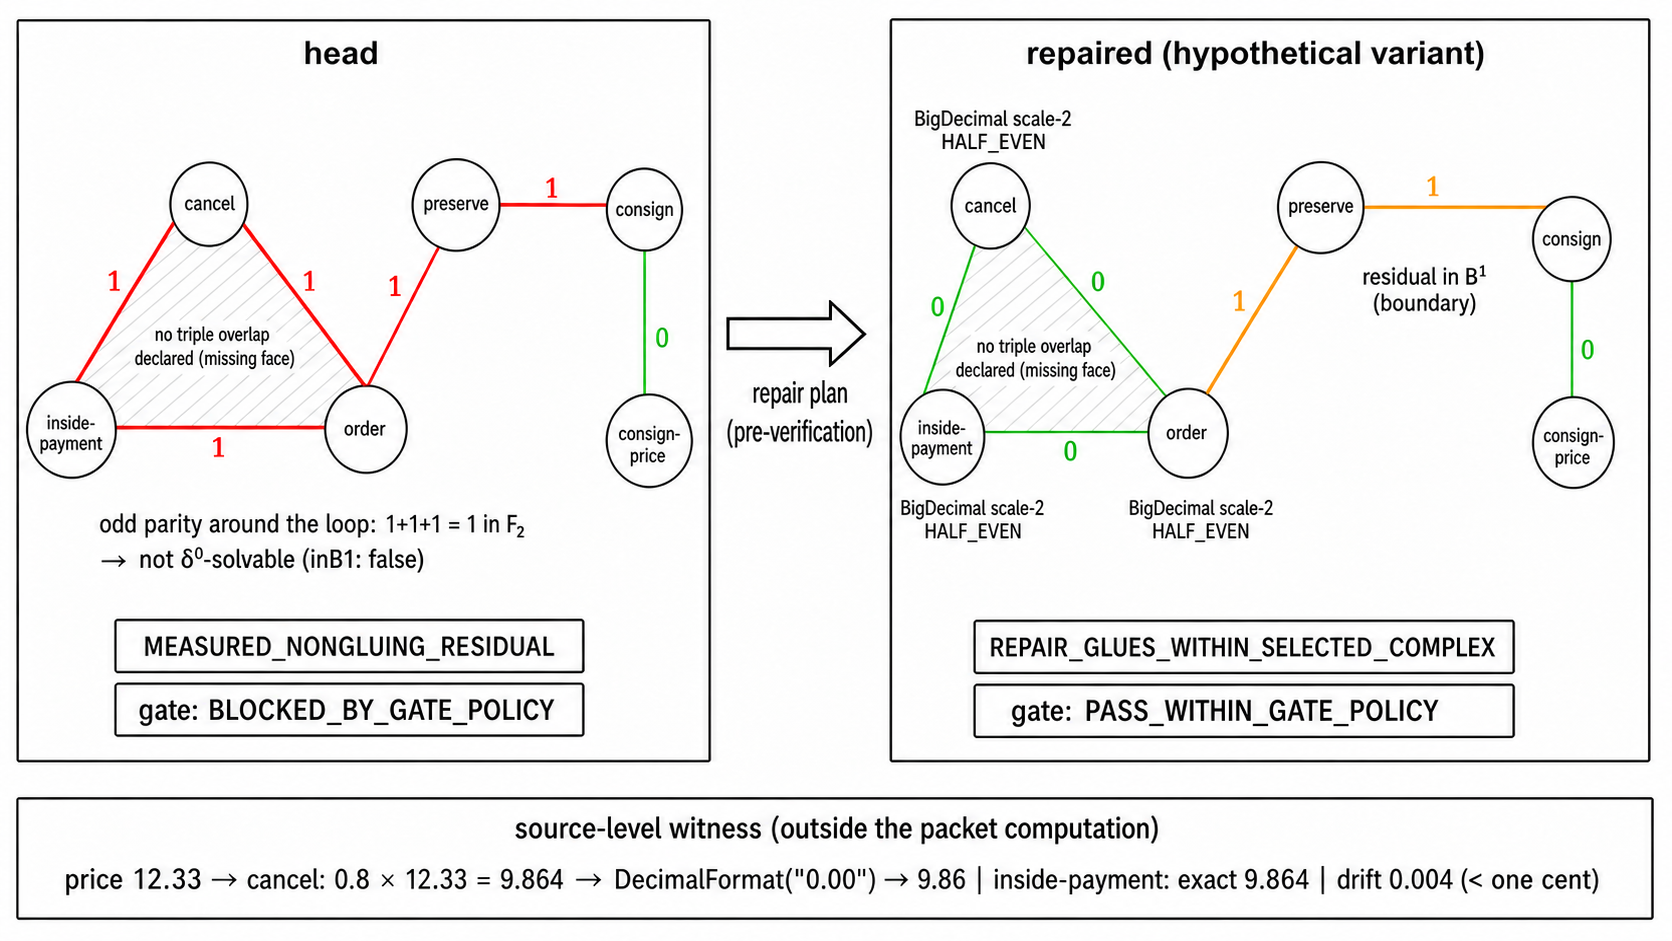
\includegraphics[width=\linewidth]{../zenodo_saga_figure2_one_cent.png}
\caption{The diagnosis staircase of the one-cent obstruction. In head
(left), derived residuals stand on the 3 triangle edges and the 2
preserve-family edges, and the odd parity on the closed loop of the
triangle is not solvable by $\delta^0$ (\code{inB1: false}). No triple
overlap is declared; the absence of the face is shown hatched. In the
repaired variant (right), replacing the 3 charts of the triangle by a
unified BigDecimal scale-2 \code{HALF\_EVEN} convention removes the
triangle residuals, and the remaining preserve-family residual falls
inside $B^1$. The numerical witness in the lower band is a
source-level recomputation by the operator and does not appear in the
packet computation (\S\ref{sec:71}).}
\label{fig:onecent}
\end{figure}

\subsection{What the measurement showed}\label{sec:73}

\paragraph{Reality of locally consistent, globally non-gluing.}
The \code{measured\_zero} of grounding says, as measurement, that each
chart satisfies its own local equations (in the sense of the
displayed-equation check of \S\ref{sec:74}). Cancel is faithful to
cancel's rounding convention, inside-payment to exact arithmetic,
order to pass-through storage. Each pairwise handoff holds as well.
What was observed as measurement is that the odd parity of the
convention mismatch is not solvable by $\delta^0$ on the closed loop
(\code{inB1: false}). Under the assertion of the absence of a face
(triple) filling the loop (\S\ref{sec:71}), this measurement becomes
an instance --- not artificially planted, but found in real OSS --- of
the central SAGA structure: locally consistent, globally non-gluing.

\paragraph{Every step of the staircase works on derived residuals alone.}
From the measurement of non-boundary residuals derived from
observation (ArchMap) and law / equations (law surfaces,
MeasurementProfile), through blocking by the gate, prior verification
of the repair plan, the recording by compare of the disappearance of
the obstruction and of the residual difference of the run pair, to
gate PASS --- the full circle was walked without supplying any
authored residuals, certificates, or comparison data. The only operator
declarations that remain are the selected complex (\S\ref{sec:74})
and the repaired variant.

\paragraph{Effectiveness of the mathematical discipline.}
Declaring the drift-bearing triangle itself as a triple is rejected by
the cocycle condition --- a mathematically legitimate rejection.
Mismatches without witness bindings and references without grounds
were rejected fail-closed. The discipline held under the load of real data.

\paragraph{Executed silence.}
The measurement axis requiring runtime measured values (axis name
\code{harmonic-debt}) was not supplied in the absence of actual
measurements and was treated as silence. Likewise, not emitting class
vocabulary on a complex without triple declarations is the same
discipline in action; ArchSig recorded that boundary as a named
boundary statement, minimally, near the conclusion.

\subsection{Input contract and computation}\label{sec:74}

We now fix the input contract and the computation on which the
diagnosis above stands. The inputs of ArchSig are the following
artifacts.
\begin{itemize}
\item \textbf{ArchMap}: the Atom observation of the target system.
Records charts (local contexts), section values, and the
correspondence of overlaps.
\item \textbf{LawPolicy} (artifact name): fixes the Atom vocabulary in
use and the selected equation reading.
\item \textbf{law surface} (artifact name): the family of equation
surfaces used by the diagnosis (closed-equational, SAGA-grounded,
descent). The descent surface includes the declarations of witness
variables bound to mismatch edges.
\item \textbf{MeasurementProfile}: fixes the conditions of
measurement, including the coefficient (in this case study,
\code{F2}).
\item \textbf{repair plan}: declares only the selected complex
(charts, overlaps, optional triple overlaps, enumeration assertion)
and a reference to the target cover. It carries no residuals, no
coefficients, no comparison data.
\end{itemize}

The charts and overlaps of the repair plan are references into the
observation; declarations that do not resolve to an observed cover and
observed restrictions are not accepted. The remaining enumeration
assertion and the presence or absence of triple-overlap declarations
are author assertions: they accompany the conclusions as disclosure
rows of the assumption ledger, not as material from which conclusions
are derived (\S\ref{sec:76}). Thus the only thing the repair plan adds
of its own is disclosed assumptions.

Residuals are not inputs. ArchSig's \code{analyze} computes the
following and emits them as a measurement packet.
\begin{itemize}
\item Per-chart \textbf{grounding}: whether each chart passes the
displayed-equation check. The check targets the defect coordinates
selected by the law surface (the residuals of displayed equations, the
finite realization of the $\epsilon$ of \S\ref{sec:34}) and the
declared criteria --- not ``complete fulfillment of all equations on
the chart''.
\item Per-overlap \textbf{residual derivation}: derives an \code{F2}
value from the comparison of the section-value sets observed by the
two end charts of each edge of the selected cover, recording per edge
the provenance of the law surface's witness binding and the observed
atom references. A witness binding is a per-edge declaration
connecting a mismatch to a law-side violation coordinate (the finite
realization of the $\nu$ of \S\ref{sec:34}); it carries no instance
values. A mismatch without a binding has no law-side coordinate on
which the derived residual could stand, so it falls fail-closed to
non-computability.
\item \textbf{Boundary membership} on the selected 1-skeleton: the
finite \code{F2} computation of whether the derived residual belongs
to the $\delta^0$-image ($B^1$). The vocabulary of residual classes is
unlocked only when a triple overlap is declared on the connected
component where the residual stands and the cocycle check actually
runs. On components without triple declarations the selected $C^2$ is
zero and the cocycle condition holds automatically, so ArchSig emits
no class vocabulary and makes that boundary explicit in the packet as
a named boundary statement.
\end{itemize}

\code{compare} confronts the packets of two runs and records the
change in the obstruction together with the reading of the run pair.
The reading of the run pair is the finite \code{F2} decision of
whether the difference of the derived residuals of the two runs
belongs to $\operatorname{im}\delta^0$ on the selected $C^1$.
\code{gate} returns the verdict \code{PASS\_WITHIN\_GATE\_POLICY} or
\code{BLOCKED\_BY\_GATE\_POLICY} from a packet and a gate policy.

We fix the correspondence between the three law surfaces and the
outputs. The closed-equational surface declares the per-edge equations
of convention agreement and carries the detection of mismatches (the
\code{cech} stage). The SAGA-grounded surface declares the per-chart defect
coordinates and criteria and carries grounding. The descent surface
declares the witness bindings on mismatch edges and carries residual
derivation and boundary membership (the \code{saga-descent} stage). The
``stages'' mentioned by the condition matrix of \S\ref{sec:76} and its
note~1 refer to this correspondence.

What this computation executes is a finite fragment of the complex
vocabulary of Section~\ref{sec:4}: residual derivation on the selected
1-skeleton, $B^1$ membership, and the residual difference of a run
pair reduce to finite \code{F2} linear algebra. The finite
instantiation of the comparison of Theorem~\ref{thm:central} ($\chi$,
$\Phi$, $\kappa$, presentation exactness) is not within the scope of
this computation; it is carried by the Lean witnesses of
Section~\ref{sec:6} (\S\ref{sec:77}).

Under this contract, the measurement claim of this paper stands on the
following. \textbf{The conclusions of the SAGA diagnosis --- residuals,
boundary membership, gate verdicts --- are derived deterministically
from the Atom observation and the selected equation system. What the
operator can write are choices: the scope of observation, the selected
complex, the witness bindings; no input carrying conclusions exists in
this contract.} This separation is enforced by fail-closed checks:
charts outside the selected cover, overlaps without observed
restrictions, duplicated overlap declarations, unobserved sections,
and mismatches without witness bindings all stop the computation
without generating conclusions. Therefore, while obstructions can be
silenced by selection (enumeration completeness is disclosed as an
assumption in \S\ref{sec:76}), no nonzero residual can be erected on
an edge where the observations agree.

\subsection{Supplying the inputs: authoring of observation and reproducibility}\label{sec:75}

Supplying an ArchMap involves semantic reading of how the sources are
used. This reading is a probabilistic process and cannot be replaced
by a deterministic computation. This work does not hide that stage; it
fixes it as a process. That is, the creation of the ArchMap is defined
as a fixed procedure executed by an AI agent --- hereafter the
\textbf{authoring SKILL} --- turning the probabilistic reading into a
traceable artifact.

The SKILL fixes the provenance of observation by the following
discipline.
\begin{itemize}
\item \textbf{Separation of the mechanical layer and the reading
layer}: the mechanical layer performs only file enumeration, content
hashing, literal comparison of normalized keys, and referential
integrity checks. Generation of Atoms, semantic choices, adoption or
rejection of candidates, and similarity-based merging are not
permitted in the mechanical layer; they remain as recorded judgments
of the reading layer.
\item \textbf{Approval record of scope}: the revision of the target
repository, the include / exclude globs, and the approved scope
manifest are fixed as artifacts. Observation claims are bounded by the
recorded revision and the selected scope; extraction of all evidence
is not claimed.
\item \textbf{Independent two-pass reading and adjudication}: the
standard mode (full-dual) reads the same worklist twice independently,
takes an extraction diff, and adjudicates discrepancies by re-reading
the sources. Adoption decisions are recorded with counts and grounds.
\item \textbf{Authoring audit}: the integrated ArchMap becomes a
measurement input only after passing mechanical checks (referential
integrity, coverage ledger, and so on).
\item \textbf{Run records and explicit models}: each authoring run
records the model used. The ArchMap of all 42 services underlying this
case study (2{,}118 atoms / 43 contexts / 440 sources) was created by
a run whose extraction and adjudication subagents were pinned to a
lightweight model. The fact that observation supply does not demand an
expensive frontier model has thus been measured as a practical
condition of this measurement system.
\end{itemize}

Under this process design, reproducibility splits into two layers.
ArchSig's computation is deterministic: the same input artifacts
return the same outputs (verified by digests). The generation of the
ArchMap is probabilistic, but since scope, grounds, procedure,
adjudication, and audit are fixed in artifacts, a third party can
re-execute the observation under the same discipline and confront the
results. Chaining the probabilistic semantic reading and the
deterministic measurement in series is the design principle of this
supply pipeline.

\subsection{Conditions and input kinds: the condition matrix}\label{sec:76}

Table~\ref{tab:conditionmatrix} fixes, for each conclusion of the
diagnosis staircase, under which kind of condition it stands. \code{computed}
denotes a finite computation from the inputs; \code{checked} a
condition checked by ArchSig against finite artifacts; \code{assumed}
a premise declared by the author or the profile and recorded by the
packet in the assumption ledger; \code{unmeasured} an axis not
supplied and kept silent. The head and repaired packets record the
same distinctions.

\begin{table}[htbp]
\centering
\scriptsize
\begin{tabular}{@{}p{0.20\textwidth}p{0.17\textwidth}p{0.13\textwidth}p{0.42\textwidth}@{}}
\toprule
Condition & Kind & Status & Record \\
\midrule
finite cover & property of finite artifacts & \code{checked} & site
cover digest computed and recorded from normalized contexts, covers,
and the derived nerve \\
\addlinespace
residual derivation & comparison of observed sections &
\code{computed} & per-edge \code{F2} values, witness bindings, and
provenance of observed atom references; in head, the 3 triangle edges
+ 2 preserve edges mismatch \\
\addlinespace
witness bindings & law surface declaration & \code{checked} & mismatch
edges require witness variable bindings; unbound mismatches fall
fail-closed to non-computability \\
\addlinespace
coefficient (\code{F2}) & law-side selection & \code{checked} &
declaration of the selected MeasurementProfile; the repair plan
carries no coefficients \\
\addlinespace
enumeration completeness of the selected complex & author assertion &
\code{assumed} & the repair plan's enumeration assertion recorded as
an assumption ledger row \\
\addlinespace
triple absence / class vocabulary & author assertion & \code{assumed}
(class vocabulary not unlocked) & the selected complex declares no
triples (\S\ref{sec:71}); the reading stays at 1-skeleton boundary
membership, and a named boundary statement makes the boundary explicit \\
\addlinespace
boundary membership & finite \code{F2} computation & \code{computed} &
head: \code{inB1: false}; repaired: \code{inB1: true} \\
\addlinespace
U-adequacy, Leray-type comparison & profile-supplied premises &
\code{assumed} & U-adequacy is the premise that the selected cover
suffices for the target reading; Leray-type comparison is the premise
needed to compare the cover-relative reading with cover-independent
sheaf cohomology. Both are disclosed as ledger rows, and the latter
comparison is not claimed (\S\ref{sec:57}) \\
\addlinespace
torsor property, fixedness of the action, coefficient descent &
profile-supplied premises & \code{assumed} & the three premises for
reading local sections as torsors of the coefficient (torsor property
of local sections, fixedness of the action, descent of the
coefficient); 3 ledger rows \\
\addlinespace
restriction surjectivity & profile-supplied premise & \code{assumed} &
the premise that restriction maps are surjective onto overlaps; ledger
row \\
\addlinespace
forest nerve & profile-supplied premise & \code{assumed} (not
satisfied in this packet) & the ledger records the forest premise, and
the nerve computation of the same packet shows 1 cycle as
\code{computed} (note~1) \\
\addlinespace
quotient sheaf condition & law surface declaration & \code{assumed} &
the law-surface-side declaration that the coefficient system playing
the role of the quotient coefficient satisfies the sheaf condition;
disclosed as a ledger row \\
\addlinespace
residual difference of the run pair (head$\leftrightarrow$repaired) &
derived reading on the run pair & \code{computed} & $\delta^0$
solvability of the difference of the derived residuals of the two runs
(\S\ref{sec:74}); for this pair the difference is not solvable by
$\delta^0$ \\
\addlinespace
repaired ArchMap & hypothetical repair input & supplied /
hypothetical & a hypothesis variant expressing the unified convention;
\code{PASS\_WITHIN\_GATE\_POLICY} does not indicate an implemented
repair \\
\addlinespace
runtime monetary magnitude & empirical measurement & \code{unmeasured}
& \code{harmonic-debt} not supplied; silence. Frequency and amounts
are not included in the conclusions \\
\bottomrule
\end{tabular}
\caption{Condition matrix: each conclusion of the diagnosis staircase
and the kind of condition under which it stands.}
\label{tab:conditionmatrix}
\end{table}

Note 1: the forest nerve is a disclosed unsatisfied premise. The
nonzero reading of the \code{saga-descent} stage in head (the $B^1$
membership decision) does not depend on this row. The verdict of the
\code{cech} stage separately declares its dependence on this assumption.

\subsection{Boundary of the claims}\label{sec:77}

The claims of this case study are limited to the following scope. The
detection of the convention mismatch itself was carried by the stage
of the closed-equational surface. What the SAGA stage added is: the
descent reading of the same observation as boundary membership on the
selected 1-skeleton; the explicit limitation of the grounding reading
(\S\ref{sec:73}); the prior verification of the repair plan; the
reading of the residual difference of the run pair (\S\ref{sec:74});
and the consistent diagnosis of the gate. We do not claim that ``SAGA
discovered a new failure''.

What is authored is selection. The selected complex (repair plan), the
witness bindings (law surface), and the repaired variant are
declarations written by the operator, and none of them carries
residual values. Class vocabulary is not unlocked: in this packet,
where no triple is declared on the component containing the triangle,
ArchSig's reading stays at boundary membership (\S\ref{sec:76}). The
repaired variant is a hypothetical-repair ArchMap with rewritten
sections, and what \code{PASS\_WITHIN\_GATE\_POLICY} shows is the
mechanism of prior verification --- ``with this repair proposal, the
system would glue''. The frequency of the drift and its monetary
magnitude require runtime measurement and are not measured in this
paper. Broad benchmark evaluation and general detection performance
are matters for separate empirical studies.

The finite instantiation of Theorem~\ref{thm:central} is outside the
scope of this case study. Its bearer is the Lean witness of
Section~\ref{sec:6} (the circle witness of Example~\ref{ex:circle});
what the packet of this section carries are the finite checks shown by
the condition matrix of \S\ref{sec:76}. No correspondence transporting
the measurement run into Lean is required.

We also make explicit the coverage of the SKILL-based supply process. The authoring SKILL of \S\ref{sec:75} covers the
supply of the ArchMap, and an authoring SKILL of the same kind is in
place for the selected complex (repair plan). The law surfaces and the
repaired variant were supplied, at the time of this experiment, as
builder scripts and authored declarations. The builder scripts and
supply findings of this experiment are recorded as design material for
that step.

\subsection{Reproduction}\label{sec:78}

All input artifacts, primary outputs, builder scripts, and the
authoring SKILL itself are included in the reproduction bundle. The
schema versions of the artifacts (for the repair plan,
\code{archsig-repair-plan/v0.5.7}) are fixed by the bundle manifest.
The \code{inputDigests} of the primary outputs have been verified to
agree with the canonical digests. Reproduction consists of executing
\code{analyze} (head / repaired), \code{compare}, and \code{gate}
$\times2$ from the fixed ArchSig version and inputs, and confirming
agreement of the runIds and the gate verdicts.

\textbf{TODO:} fix the relative paths within the deposit, the ArchSig
version, the full set of execution commands, and the expected outputs
once the release identity is finalized. (The current canonical
reproduction procedure is
\code{docs/reports/train\_ticket\_dogfooding/saga\_diagnosis.md}.)
